% ============================================================
%  يُترجَم بـ XeLaTeX  (في Overleaf: Menu → Compiler → XeLaTeX)
%  الخط: Amiri (متوفر في Overleaf، أو حمّله من github.com/aliftype/amiri)
% ============================================================
\documentclass[12pt,a4paper]{article}
\usepackage[a4paper,margin=1.7cm,top=2.3cm,bottom=2.9cm,headheight=15pt,footskip=1.5cm]{geometry}
\usepackage{amsmath,amssymb}
\usepackage{icomma}
\usepackage[english,bidi=default,layout=lists]{babel}
\babelprovide[import,main]{arabic}
\babelfont{rm}[Scale=1.08]{Amiri}
\babelfont{sf}[Scale=1.08]{Amiri}
\usepackage[most]{tcolorbox}
\usepackage{tikz}
\usetikzlibrary{arrows.meta,calc,shadings}
\usepackage{array}
\usepackage{colortbl}
\usepackage{fancyhdr}
\usepackage{titlesec}
\usepackage{enumitem}
\usepackage{collcell}
\usepackage{needspace}
\usepackage{etoolbox}
% أعمدة جداول تُكتب خلاياها بالعربية في الاتجاه الصحيح
\newcolumntype{C}{>{\collectcell\ar}c<{\endcollectcell}}
% تجنب عنوان يتيم في أسفل الصفحة
\pretocmd{\section}{\Needspace{15\baselineskip}}{}{}
\pretocmd{\subsection}{\Needspace{11\baselineskip}}{}{}

% ---------- الألوان ----------
\definecolor{cDef}{HTML}{1F4E9C}
\definecolor{cThm}{HTML}{B3261E}
\definecolor{cRem}{HTML}{2E7D32}
\definecolor{cEx}{HTML}{C76B00}
\definecolor{cMeth}{HTML}{6A1B9A}
\definecolor{cSol}{HTML}{00695C}
\definecolor{cSec}{HTML}{1F3A68}

% ---------- العناوين ----------
\titleformat{\section}{\Large\bfseries\color{cSec}}{\thesection.}{0.6em}{}[{\color{cSec!60}\titlerule[1pt]}]
\titleformat{\subsection}{\large\bfseries\color{cThm!85!black}}{\thesubsection.}{0.5em}{}
\titlespacing*{\section}{0pt}{14pt}{8pt}
\titlespacing*{\subsection}{0pt}{10pt}{5pt}
\setlength{\parindent}{0pt}
\setlength{\parskip}{4pt}
\setlist{itemsep=2pt,topsep=3pt}

% ---------- الصناديق (تُرسم في سياق LTR ويُكتب محتواها بالعربية) ----------
\newtcolorbox{arbox}[3][]{enhanced,
  colback=#2!5,colframe=#2!80!black,arc=2mm,boxrule=0.8pt,
  left=6pt,right=6pt,top=8pt,bottom=5pt,
  fonttitle=\bfseries,coltitle=white,
  title={\foreignlanguage{arabic}{#3}},
  attach boxed title to top right={xshift=-5mm,yshift=-3mm},
  boxed title style={colback=#2!80!black,arc=1.5mm,boxrule=0pt},
  before upper={\selectlanguage{arabic}},
  before skip=8pt,after skip=8pt,breakable,#1}
\newenvironment{BOX}[2]{\begin{otherlanguage}{english}\begin{arbox}{#1}{#2}}{\end{arbox}\end{otherlanguage}}
\newenvironment{tarif}[1][تعريف]{\begin{BOX}{cDef}{#1}}{\end{BOX}}
\newenvironment{khassia}[1][خاصية]{\begin{BOX}{cThm}{#1}}{\end{BOX}}
\newenvironment{molahada}[1][ملاحظة]{\begin{BOX}{cRem}{#1}}{\end{BOX}}
\newenvironment{mithal}[1][مثال]{\begin{BOX}{cEx}{#1}}{\end{BOX}}
\newenvironment{tariqa}[1][طريقة]{\begin{BOX}{cMeth}{#1}}{\end{BOX}}

% ---------- التمارين والحلول ----------
\newcounter{exo}
\newenvironment{tamrin}[1]{\stepcounter{exo}\begin{BOX}{cSec}{التمرين \theexo: #1}}{\end{BOX}}
\newenvironment{hal}{\Needspace{12\baselineskip}\begin{otherlanguage}{english}\begin{arbox}[breakable]{cSol}{حل التمرين \theexo}}{\end{arbox}\end{otherlanguage}}

% رسومات TikZ تُوضع في سياق LTR
\newenvironment{LTR}{\begin{otherlanguage}{english}}{\end{otherlanguage}}
\newcommand{\ar}[1]{\foreignlanguage{arabic}{#1}}

% ---------- رموز ----------
% نقاط الحذف داخل الرياضيات (\dots يسبب خللاً في الاتجاه مع babel)
\renewcommand{\dots}{\mathinner{\ldotp\ldotp\ldotp}}
\renewcommand{\ldots}{\mathinner{\ldotp\ldotp\ldotp}}
\renewcommand{\cdots}{\mathinner{\cdotp\cdotp\cdotp}}
\newcommand{\N}{\mathbb{N}}
\newcommand{\Z}{\mathbb{Z}}
\newcommand{\D}{\mathbb{D}}
\newcommand{\Q}{\mathbb{Q}}
\newcommand{\R}{\mathbb{R}}
\newcommand{\pgcd}{\operatorname{PGCD}}
\newcommand{\ppcm}{\operatorname{PPCM}}

% ---------- تمثيل مجال على مستقيم عددي ----------
% \NLseg{a}{b}{[}{]}  مجال محدود
\newcommand{\NLseg}[4]{\begin{LTR}\begin{tikzpicture}[baseline=-0.6ex]
 \draw[-{Stealth[length=2mm]},gray!70](0,0)--(3.4,0);
 \draw[line width=2pt,cThm!80!black](0.7,0)--(2.7,0);
 \node[cThm!80!black,font=\LARGE] at (0.7,0){$#3$};
 \node[cThm!80!black,font=\LARGE] at (2.7,0){$#4$};
 \node[below=3pt,font=\footnotesize] at (0.7,0){$#1$};
 \node[below=3pt,font=\footnotesize] at (2.7,0){$#2$};
\end{tikzpicture}\end{LTR}}
% \NLright{a}{[}  مجال نحو +∞
\newcommand{\NLright}[2]{\begin{LTR}\begin{tikzpicture}[baseline=-0.6ex]
 \draw[-{Stealth[length=2mm]},gray!70](0,0)--(3.4,0);
 \draw[line width=2pt,cThm!80!black](1.3,0)--(3.3,0);
 \node[cThm!80!black,font=\LARGE] at (1.3,0){$#2$};
 \node[below=3pt,font=\footnotesize] at (1.3,0){$#1$};
\end{tikzpicture}\end{LTR}}
% \NLleft{b}{]}  مجال نحو −∞
\newcommand{\NLleft}[2]{\begin{LTR}\begin{tikzpicture}[baseline=-0.6ex]
 \draw[-{Stealth[length=2mm]},gray!70](0,0)--(3.4,0);
 \draw[line width=2pt,cThm!80!black](0.05,0)--(2.1,0);
 \node[cThm!80!black,font=\LARGE] at (2.1,0){$#2$};
 \node[below=3pt,font=\footnotesize] at (2.1,0){$#1$};
\end{tikzpicture}\end{LTR}}

% ---------- أيقونات مواقع التواصل (مرسومة بـ TikZ، لا تحتاج أي حزمة) ----------
\definecolor{cFB}{HTML}{1877F2}
\definecolor{cTG}{HTML}{229ED9}
\definecolor{cIG1}{HTML}{FEDA75}
\definecolor{cIG2}{HTML}{D62976}
\definecolor{cIG3}{HTML}{4F5BD5}
\newcommand{\fbicon}{\begin{LTR}\begin{tikzpicture}[baseline=-0.75ex,x=1em,y=1em]
 \fill[cFB] (0,0) circle (0.55);
 \node[white,inner sep=0,font=\usefont{TU}{lmss}{bx}{n}\small] at (0.04,-0.02) {f};
\end{tikzpicture}\end{LTR}}
\newcommand{\igicon}{\begin{LTR}
\begin{tikzpicture}[baseline=-0.75ex,x=1em,y=1em]
 \shade[lower left=cIG1,lower right=cIG2,upper left=cIG2,upper right=cIG3,rounded corners=0.28em] (-0.55,-0.55) rectangle (0.55,0.55);
 \draw[white,line width=0.09em,rounded corners=0.18em] (-0.36,-0.36) rectangle (0.36,0.36);
 \draw[white,line width=0.09em] (0,0) circle (0.17);
 \fill[white] (0.22,0.22) circle (0.05);
\end{tikzpicture}\end{LTR}}
\newcommand{\tgicon}{\begin{LTR}
\begin{tikzpicture}[baseline=-0.75ex,x=1em,y=1em]
 \fill[cTG] (0,0) circle (0.55);
 \fill[white] (-0.33,0.0) -- (0.32,0.27) -- (0.2,-0.3) -- (0.0,-0.15) -- (-0.08,-0.28) -- (-0.08,-0.08) -- cycle;
 \fill[cTG!70!black] (-0.08,-0.08) -- (0.25,0.2) -- (0.0,-0.15) -- (-0.08,-0.28) -- cycle;
\end{tikzpicture}\end{LTR}}
% سطر مواقع التواصل أسفل كل صفحة
% (يُكتب السطر بترتيب بصري من اليسار إلى اليمين: الأيقونة يمين كل اسم)
\newcommand{\PageBox}{\begin{LTR}\tikz[baseline=(p.base)]\node[fill=black,text=white,inner sep=2.5pt,minimum width=1.6em,minimum height=1.3em,font=\usefont{TU}{lmss}{bx}{n}\small](p){\ifnum\value{page}<10 0\fi\arabic{page}};\end{LTR}}
\newcommand{\SocialRow}{\begin{otherlanguage}{english}%
 \ar{\textbf{الأستاذ سوايسية هشام للرياضيات}}\ \tgicon\hfill
 \textbf{prof\_hicham\_math}\ \igicon\hfill
 \ar{\textbf{الأستاذ سوايسية هشام للرياضيات}}\ \fbicon\hspace{2.2em}\PageBox\end{otherlanguage}}

% ---------- رأس وتذييل الصفحة ----------
\pagestyle{fancy}
\fancyhf{}
\renewcommand{\headrulewidth}{0.6pt}
\renewcommand{\footrulewidth}{0.4pt}
% \SetHeader{يمين الرأس}{يسار الرأس}{يمين التذييل}{يسار التذييل}
\newcommand{\SetHeader}[2]{%
 \fancyhead[C]{\parbox{\textwidth}{\ar{#1\hfill #2}}}%
 \fancyfoot[C]{\parbox{\textwidth}{\small\SocialRow}}}

\pretocmd{\section}{\Needspace{24\baselineskip}}{}{}

% معلم بشبكة: \Grid{xmin}{xmax}{ymin}{ymax}
\newcommand{\Grid}[4]{%
 \draw[gray!25] (#1,#3) grid (#2,#4);
 \draw[-{Stealth}] (#1-0.2,0)--(#2+0.3,0) node[below]{$x$};
 \draw[-{Stealth}] (0,#3-0.2)--(0,#4+0.3) node[left]{$y$};
 \node[below left,font=\scriptsize] at (0,0){$O$};}

\SetHeader{\small\bfseries\color{cSec}الوحدة الأولى: الدوال العددية -- سلسلة تمارين}{\small\color{cSec}السنة الثانية ثانوي -- الشعب العلمية}

\begin{document}

\begin{LTR}
\begin{tcolorbox}[enhanced,colback=cSec,colframe=cSec,arc=3mm,halign=center,
  boxrule=0pt,top=10pt,bottom=10pt,before upper={\selectlanguage{arabic}}]
{\color{white}\Huge\bfseries سلسلة تمارين مع الحلول المفصلة}\\[6pt]
{\color{white}\large الوحدة الأولى: الدوال العددية -- السنة الثانية ثانوي}\\[4pt]
{\color{white!85!cSec}\normalsize إعداد: الأستاذ سوايسية هشام}
\end{tcolorbox}
\end{LTR}

\begin{molahada}[توجيهات]
التمارين مرتبة حسب محاور الوحدة، ثم تمرينان شاملان في الأخير. حاول حل كل تمرين بنفسك قبل الاطلاع على حله.
\end{molahada}

% =================================================================
\section{مجموعة التعريف والعمليات على الدوال}
% =================================================================
\begin{tamrin}{مجموعة التعريف}
عيّن مجموعة تعريف كل دالة من الدوال التالية:
\[f_1(x)=\frac{2x+1}{x^2-4}\qquad f_2(x)=\sqrt{3-2x}\qquad f_3(x)=\frac{1}{\sqrt{x+1}}\]
\[f_4(x)=\frac{\sqrt{x-1}}{x-3}\qquad\qquad f_5(x)=\frac{x}{x^2+1}\]
\end{tamrin}
\begin{hal}
\begin{itemize}
\item $f_1$: \ $x^2-4\ne0\iff x\ne-2$ و $x\ne2$ ، إذن $\boxed{D_{f_1}=\R-\{-2;2\}}$.
\item $f_2$: \ $3-2x\ge0\iff x\le\dfrac32$ ، إذن $\boxed{D_{f_2}=\left]-\infty;\dfrac32\right]}$.
\item $f_3$: \ $x+1>0\iff x>-1$ ، إذن $\boxed{D_{f_3}=]-1;+\infty[}$.
\item $f_4$: \ $x-1\ge0$ و $x-3\ne0$ ، إذن $\boxed{D_{f_4}=[1;3[\,\cup\,]3;+\infty[}$.
\item $f_5$: \ $x^2+1\ge1>0$ لكل $x$ ، إذن $\boxed{D_{f_5}=\R}$.
\end{itemize}
\end{hal}

\begin{tamrin}{تساوي دالتين}
في كل حالة، هل الدالتان $f$ و $g$ متساويتان؟ علّل.
\begin{enumerate}
\item $f(x)=\left(\sqrt{x+2}\right)^2$ \quad و \quad $g(x)=x+2$.
\item $f(x)=\dfrac{1}{\sqrt x-1}$ \quad و \quad $g(x)=\dfrac{\sqrt x+1}{x-1}$.
\end{enumerate}
\end{tamrin}
\begin{hal}
\begin{enumerate}
\item $D_f=[-2;+\infty[$ و $D_g=\R$. مجموعتا التعريف مختلفتان، إذن $\boxed{f\ne g}$ (رغم أن $f(x)=g(x)$ على $[-2;+\infty[$).
\item $f$: $x\ge0$ و $\sqrt x\ne1$ ، أي $D_f=[0;1[\,\cup\,]1;+\infty[$. \quad $g$: $x\ge0$ و $x\ne1$ ، أي $D_g=D_f$.\\
ومن أجل كل $x$ من $D_f$: \ $g(x)=\dfrac{\sqrt x+1}{\left(\sqrt x-1\right)\left(\sqrt x+1\right)}=\dfrac{1}{\sqrt x-1}=f(x)$ ، إذن $\boxed{f=g}$.
\end{enumerate}
\end{hal}

\begin{tamrin}{العمليات على الدوال}
$f$ و $g$ دالتان معرفتان على $\R$ بـ: \ $f(x)=x^2+1$ \ و \ $g(x)=x+2$.\\
عرّف كلاً من الدوال: \ $f+3$ ، \ $-2f$ ، \ $f+g$ ، \ $f\times g$ ، \ $\dfrac fg$.
\end{tamrin}
\begin{hal}
\begin{itemize}
\item $(f+3)(x)=x^2+4$ \ و \ $(-2f)(x)=-2x^2-2$ \ و \ $(f+g)(x)=x^2+x+3$ \ ؛ \ كلها معرفة على $\R$.
\item $(f\times g)(x)=\left(x^2+1\right)(x+2)=x^3+2x^2+x+2$ \ معرفة على $\R$.
\item $\dfrac fg$ معرفة لما $g(x)\neq0$ أي $x\ne-2$: \quad $\left(\dfrac fg\right)(x)=\dfrac{x^2+1}{x+2}$ \ على $\R-\{-2\}$.
\end{itemize}
\end{hal}

% =================================================================
\section{تركيب الدوال واتجاه التغير}
% =================================================================
\begin{tamrin}{تركيب دالتين}
$f(x)=x^2+1$ معرفة على $\R$ ، و $g(x)=\dfrac{1}{x-2}$ معرفة على $\R-\{2\}$.
\begin{enumerate}
\item اكتب كلاً من $f$ و $g$ على شكل مركب دالتين مرجعيتين.
\item عيّن مجموعة تعريف $g\circ f$ ثم احسب $(g\circ f)(x)$.
\item عيّن مجموعة تعريف $f\circ g$ ثم احسب $(f\circ g)(x)$. ماذا تلاحظ؟
\end{enumerate}
\end{tamrin}
\begin{hal}
\begin{enumerate}
\item $f=v_1\circ u_1$ حيث $u_1(x)=x^2$ و $v_1(x)=x+1$ ؛ \quad $g=v_2\circ u_2$ حيث $u_2(x)=x-2$ و $v_2(x)=\dfrac1x$.
\item $g\circ f$ معرفة إذا كان $f(x)\in D_g$ أي $x^2+1\ne2$ أي $x\ne1$ و $x\ne-1$.\\
$D_{g\circ f}=\R-\{-1;1\}$ \quad و \quad $(g\circ f)(x)=\dfrac{1}{x^2+1-2}=\boxed{\dfrac{1}{x^2-1}}$.
\item $f\circ g$ معرفة إذا كان $x\in D_g$ (لأن $D_f=\R$) ، أي $D_{f\circ g}=\R-\{2\}$:
\[(f\circ g)(x)=\frac{1}{(x-2)^2}+1=\frac{1+(x-2)^2}{(x-2)^2}=\boxed{\frac{x^2-4x+5}{(x-2)^2}}\]
\textbf{نلاحظ} أن $g\circ f\ne f\circ g$.
\end{enumerate}
\end{hal}

\begin{tamrin}{تفكيك دالة واتجاه تغيرها}
\begin{enumerate}
\item فكك كل دالة إلى مركب دالتين بسيطتين: \ $f(x)=(x+2)^2+1$ \ ، \ $g(x)=\dfrac{3}{x+1}$ \ ، \ $h(x)=\left|\dfrac{2x}{5}-1\right|$.
\item $k$ الدالة المعرفة على $]-\infty;3]$ بـ: $k(x)=\sqrt{3-x}$. اكتب $k$ على شكل مركب دالتين ثم استنتج اتجاه تغيرها.
\end{enumerate}
\end{tamrin}
\begin{hal}
\begin{enumerate}
\item \begin{itemize}
\item $f=v\circ u$ حيث $u(x)=x+2$ و $v(x)=x^2+1$.
\item $g=v\circ u$ حيث $u(x)=x+1$ و $v(x)=\dfrac3x$.
\item $h=v\circ u$ حيث $u(x)=\dfrac25x-1$ و $v(x)=|x|$.
\end{itemize}
\item $k=v\circ u$ حيث $u(x)=3-x$ و $v(x)=\sqrt x$.\\
$u$ متناقصة تماماً على $]-\infty;3]$ ($-1<0$) و $u\big(]-\infty;3]\big)=[0;+\infty[$ ، و $v$ متزايدة تماماً على $[0;+\infty[$.\\
اتجاها التغير متعاكسان، إذن \textbf{$k$ متناقصة تماماً على $]-\infty;3]$}.
\end{enumerate}
\end{hal}

\begin{tamrin}{اتجاه التغير باستعمال الدوال المرجعية}
ادرس اتجاه تغير كل دالة على المجال المعطى:
\begin{enumerate}
\item $f(x)=2\sqrt x+3$ على $[0;+\infty[$.
\item $g(x)=\dfrac1x-4$ على $]-\infty;0[$.
\item $h(x)=-\dfrac{3}{x-1}+2$ على $]1;+\infty[$.
\item $k(x)=(x+1)^2$ على $]-1;+\infty[$.
\end{enumerate}
\end{tamrin}
\begin{hal}
\begin{enumerate}
\item $x\mapsto\sqrt x$ متزايدة تماماً، و $2>0$ ، ثم نضيف $3$: $f$ \textbf{متزايدة تماماً} على $[0;+\infty[$.
\item $x\mapsto\dfrac1x$ متناقصة تماماً على $]-\infty;0[$ ، وإضافة $-4$ لا تغير الاتجاه: $g$ \textbf{متناقصة تماماً}.
\item $x\mapsto\dfrac1{x-1}$ مركب $u(x)=x-1$ (متزايدة) و $\dfrac1x$ (متناقصة على $]0;+\infty[$) فهي متناقصة تماماً على $]1;+\infty[$.\\
الضرب في $-3<0$ يعكس الاتجاه، وإضافة $2$ لا تغيره: $h$ \textbf{متزايدة تماماً} على $]1;+\infty[$.
\item $u(x)=x+1$ متزايدة و $u\big(]-1;+\infty[\big)=]0;+\infty[$ حيث الدالة مربع متزايدة تماماً: $k$ \textbf{متزايدة تماماً}.
\end{enumerate}
\end{hal}

\begin{tamrin}{اتجاه تغير $\sqrt u$ و $\dfrac1u$}
ادرس اتجاه تغير كل دالة على المجال المعطى:
\begin{enumerate}
\item $f(x)=\sqrt{3-x}$ على $]-\infty;3]$.
\item $g(x)=\dfrac{1}{x^2-4x+5}$ على $\R$ ، ثم استنتج القيمة الحدية العظمى لـ $g$.
\item $h(x)=\sqrt{x^2+2x+3}$ على $\R$.
\item $k(x)=3-\dfrac{2}{\sqrt x+1}$ على $[0;+\infty[$.
\end{enumerate}
\end{tamrin}
\begin{hal}
\begin{enumerate}
\item $u(x)=3-x\ge0$ على $]-\infty;3]$ ومتناقصة تماماً ، إذن $f=\sqrt u$ \textbf{متناقصة تماماً} على $]-\infty;3]$.
\item $u(x)=x^2-4x+5=(x-2)^2+1\ge1>0$: لا تنعدم وإشارتها ثابتة. \ $u$ متناقصة تماماً على $]-\infty;2]$ ومتزايدة تماماً على $[2;+\infty[$ ، إذن $g=\dfrac1u$ \textbf{متزايدة تماماً} على $]-\infty;2]$ و\textbf{متناقصة تماماً} على $[2;+\infty[$.\\
القيمة الحدية العظمى: $\boxed{g(2)=1}$.
\item $u(x)=x^2+2x+3=(x+1)^2+2>0$ ، متناقصة تماماً على $]-\infty;-1]$ ومتزايدة تماماً على $[-1;+\infty[$ ، إذن $h=\sqrt u$ \textbf{متناقصة تماماً} على $]-\infty;-1]$ و\textbf{متزايدة تماماً} على $[-1;+\infty[$ ، وقيمتها الحدية الصغرى $h(-1)=\sqrt2$.
\item $u(x)=\sqrt x+1\ge1>0$ ومتزايدة تماماً على $[0;+\infty[$ ، إذن $\dfrac1u$ متناقصة تماماً ، والضرب في $-2<0$ يعكس الاتجاه ، وإضافة $3$ لا تغيره: $k$ \textbf{متزايدة تماماً} على $[0;+\infty[$.
\end{enumerate}
\end{hal}

% =================================================================
\section{التمثيلات البيانية}
% =================================================================
\begin{tamrin}{تمثيلات مستنتجة}
$f$ الدالة المعرفة على $\R$ بـ: $f(x)=x^2-2$.
\begin{enumerate}
\item ارسم $(C_f)$ انطلاقاً من التمثيل البياني للدالة مربع.
\item استنتج التمثيل البياني للدالة $g(x)=|f(x)|$ ، ثم للدالة $h(x)=f\big(|x|\big)$. ماذا تلاحظ؟
\end{enumerate}
\end{tamrin}
\begin{hal}
\begin{minipage}{0.55\textwidth}
\begin{enumerate}
\item $(C_f)$ صورة منحنى الدالة $x\mapsto x^2$ بالانسحاب الذي شعاعه $-2\vec j$.
\item $g(x)=f(x)$ لما $f(x)\ge0$ ، أي لما $x\le-\sqrt2$ أو $x\ge\sqrt2$ ؛ وعلى $]-\sqrt2;\sqrt2[$ يكون $(C_g)$ نظير $(C_f)$ بالنسبة لمحور الفواصل.\\[2pt]
$h(x)=f(|x|)=|x|^2-2=x^2-2=f(x)$ ، إذن $(C_h)$ ينطبق على $(C_f)$ لأن $f$ زوجية أصلاً.
\end{enumerate}
\end{minipage}\hfill
\begin{minipage}{0.42\textwidth}
\centering
\begin{LTR}
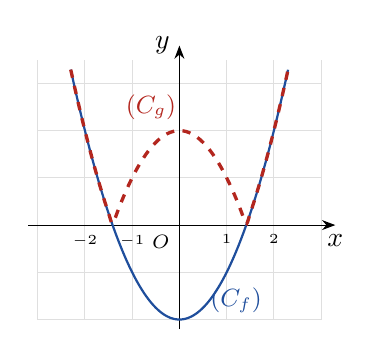
\begin{tikzpicture}[scale=0.6]
 \Grid{-3}{3}{-2}{3.5}
 \foreach \t in {-2,-1,1,2} \node[below,font=\tiny] at (\t,0){$\t$};
 \draw[cDef,thick,smooth,samples=60,domain=-2.3:2.3] plot (\x,{\x*\x-2});
 \draw[cThm,very thick,dashed,smooth,samples=80,domain=-2.3:2.3] plot (\x,{abs(\x*\x-2)});
 \node[cDef,font=\small] at (1.2,-1.6){$(C_f)$};
 \node[cThm,font=\small] at (-0.6,2.5){$(C_g)$};
\end{tikzpicture}
\end{LTR}
\end{minipage}
\end{hal}

\begin{tamrin}{منحنى مستنتج بانسحاب}
$f$ الدالة المعرفة على $\R-\{3\}$ بـ: $f(x)=\dfrac{1}{x-3}+2$.
\begin{enumerate}
\item بيّن أن $(C_f)$ صورة منحنى الدالة مقلوب بانسحاب يُطلب تعيين شعاعه.
\item استنتج اتجاه تغير $f$ ، ثم ارسم $(C_f)$.
\end{enumerate}
\end{tamrin}
\begin{hal}
\begin{minipage}{0.55\textwidth}
\begin{enumerate}
\item $f(x)=u(x-3)+2$ حيث $u(x)=\dfrac1x$ ، إذن $(C_f)$ صورة منحنى الدالة مقلوب بالانسحاب الذي شعاعه $\boxed{\vec v\binom{3}{2}}$.
\item الانسحاب لا يغير اتجاه التغير: $f$ متناقصة تماماً على $]-\infty;3[$ وعلى $]3;+\infty[$.\\
المستقيمان $x=3$ و $y=2$ صورتا المحورين، والنقطة $\Omega(3;2)$ مركز تناظر لـ $(C_f)$.
\end{enumerate}
\end{minipage}\hfill
\begin{minipage}{0.42\textwidth}
\centering
\begin{LTR}
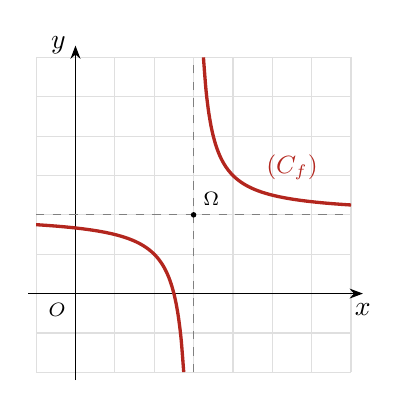
\begin{tikzpicture}[scale=0.5]
 \Grid{-1}{7}{-2}{6}
 \draw[gray,dashed] (3,-2)--(3,6); \draw[gray,dashed] (-1,2)--(7,2);
 \draw[cThm,very thick,smooth,samples=60,domain=-1:2.75] plot (\x,{1/(\x-3)+2});
 \draw[cThm,very thick,smooth,samples=60,domain=3.25:7] plot (\x,{1/(\x-3)+2});
 \fill (3,2) circle (2pt) node[above right,font=\scriptsize]{$\Omega$};
 \node[cThm,font=\small] at (5.5,3.2){$(C_f)$};
\end{tikzpicture}
\end{LTR}
\end{minipage}
\end{hal}

% =================================================================
\section{الشفعية والتناظر وتغيير المعلم}
% =================================================================
\begin{tamrin}{الشفعية}
ادرس شفعية كل دالة: \quad $f(x)=x^3-3x$ \ ، \ $g(x)=x^2+|x|$ \ ، \ $h(x)=x^2+x$.
\end{tamrin}
\begin{hal}
المجموعة $\R$ متناظرة بالنسبة لـ $0$ في الحالات الثلاث.
\begin{itemize}
\item $f(-x)=-x^3+3x=-f(x)$: $f$ \textbf{فردية} و $(C_f)$ متناظر بالنسبة لمبدأ المعلم.
\item $g(-x)=x^2+|-x|=g(x)$: $g$ \textbf{زوجية} و $(C_g)$ متناظر بالنسبة لمحور التراتيب.
\item $h(1)=2$ و $h(-1)=0$ ، إذن $h(-1)\ne h(1)$ و $h(-1)\ne-h(1)$: $h$ \textbf{ليست زوجية ولا فردية}.
\end{itemize}
\end{hal}

\begin{tamrin}{محور التناظر ومركز التناظر}
\begin{enumerate}
\item $f(x)=x^2+2x+1$. بيّن أن المستقيم ذا المعادلة $x=-1$ محور تناظر لـ $(C_f)$.
\item $g(x)=\dfrac{3x-5}{x-2}$ على $\R-\{2\}$. بيّن أن النقطة $\Omega(2;3)$ مركز تناظر لـ $(C_g)$ بطريقتين.
\end{enumerate}
\end{tamrin}
\begin{hal}
\begin{enumerate}
\item من أجل كل $x$: \ $f(-1+x)=(-1+x)^2+2(-1+x)+1=x^2$ \ و \ $f(-1-x)=x^2$.\\
إذن $f(-1+x)=f(-1-x)$ والمستقيم $x=-1$ محور تناظر لـ $(C_f)$. (فعلاً $f(x)=(x+1)^2$).
\item \textbf{الطريقة 1:} من أجل $x\ne0$: \ $g(2+x)=\dfrac{3x+1}{x}=3+\dfrac1x$ \ و \ $g(2-x)=\dfrac{1-3x}{-x}=3-\dfrac1x$.\\
ومنه $g(2+x)+g(2-x)=6=2\times3$ ، إذن $\Omega(2;3)$ مركز تناظر.\\[3pt]
\textbf{الطريقة 2:} نضع $x=X+2$ و $y=Y+3$: \ $Y+3=\dfrac{3X+1}{X}=3+\dfrac1X$ أي $Y=\dfrac1X$ ،
وهي دالة فردية، إذن $\Omega$ مركز تناظر لـ $(C_g)$.
\end{enumerate}
\end{hal}

\begin{tamrin}{تغيير المعلم}
$f(x)=x^2-4x+9$ و $\Omega(2;5)$. اكتب معادلة $(C_f)$ في المعلم $\left(\Omega;\vec i,\vec j\right)$ ، ثم استنتج طبيعة $(C_f)$ ومحور تناظره.
\end{tamrin}
\begin{hal}
دساتير تغيير المعلم: $x=X+2$ و $y=Y+5$. بالتعويض في $y=x^2-4x+9$:
\[Y+5=(X+2)^2-4(X+2)+9=X^2+4X+4-4X-8+9=X^2+5\]
إذن معادلة $(C_f)$ في المعلم الجديد: $\boxed{Y=X^2}$. الدالة $X\mapsto X^2$ زوجية، إذن $(C_f)$ قطع مكافئ رأسه $\Omega(2;5)$ ،
ومحور تناظره هو محور التراتيب الجديد، أي المستقيم ذو المعادلة $\boxed{x=2}$ في المعلم القديم.
\end{hal}

% =================================================================
\section{كثيرات الحدود والدرجة الثانية}
% =================================================================
\begin{tamrin}{تحليل كثير حدود}
$f(x)=x^3-x^2-4x+4$.
\begin{enumerate}
\item تحقق أن $2$ جذر لـ $f$.
\item عيّن الأعداد $a$ ، $b$ ، $c$ بحيث $f(x)=(x-2)\left(ax^2+bx+c\right)$ ، ثم حلّل $f(x)$ إلى جداء عوامل من الدرجة الأولى.
\item حل في $\R$ المعادلة $f(x)=0$ ثم المتراجحة $f(x)\ge0$.
\end{enumerate}
\end{tamrin}
\begin{hal}
\begin{enumerate}
\item $f(2)=8-4-8+4=0$ ، إذن $2$ جذر لـ $f$.
\item $(x-2)\left(ax^2+bx+c\right)=ax^3+(b-2a)x^2+(c-2b)x-2c$. بالمطابقة:
$a=1$ ، $b-2a=-1$ أي $b=1$ ، $-2c=4$ أي $c=-2$ (وتحقق $c-2b=-4$).\\
ومنه $f(x)=(x-2)\left(x^2+x-2\right)=\boxed{(x-2)(x-1)(x+2)}$.
\item $f(x)=0\iff x\in\{-2;1;2\}$.
\begin{center}
\renewcommand{\arraystretch}{1.4}
\begin{tabular}{|C|C|C|C|C|C|C|C|}\hline
$x$ & $-\infty$ \quad & $-2$ & & $1$ & & $2$ & \quad $+\infty$\\\hline
$x+2$ & $-$ & $0$ & $+$ & $\vert$ & $+$ & $\vert$ & $+$\\\hline
$x-1$ & $-$ & $\vert$ & $-$ & $0$ & $+$ & $\vert$ & $+$\\\hline
$x-2$ & $-$ & $\vert$ & $-$ & $\vert$ & $-$ & $0$ & $+$\\\hline
$f(x)$ & $-$ & $0$ & $+$ & $0$ & $-$ & $0$ & $+$\\\hline
\end{tabular}
\end{center}
إذن مجموعة حلول المتراجحة $f(x)\ge0$ هي: \ $\boxed{S=[-2;1]\,\cup\,[2;+\infty[}$.
\end{enumerate}
\end{hal}

\begin{tamrin}{المعادلات والمتراجحات من الدرجة الثانية}
\begin{enumerate}
\item $f(x)=x^2+3x-10$. أعط الشكل النموذجي لـ $f(x)$ ، ثم بيّن أن $f(x)\ge-\dfrac{49}{4}$ لكل $x$ ، ثم حلّل $f(x)$.
\item حل في $\R$ المعادلات: \ (أ) $2x^2+5x-3=0$ \ (ب) $-x^2+2x-5=0$ \ (ج) $x^2-8x+16=0$.
\item حل في $\R$ المتراجحات: \ (أ) $-3x^2+4x-1>0$ \ (ب) $2x^2-2x-4\le0$ \ (ج) $x^2-2\sqrt3\,x+3\le0$.
\end{enumerate}
\end{tamrin}
\begin{hal}
\begin{enumerate}
\item $f(x)=\left(x+\dfrac32\right)^2-\dfrac94-10=\boxed{\left(x+\dfrac32\right)^2-\dfrac{49}{4}}$ ، وبما أن المربع موجب فإن $f(x)\ge-\dfrac{49}4$.\\
$f(x)=\left(x+\dfrac32-\dfrac72\right)\left(x+\dfrac32+\dfrac72\right)=\boxed{(x-2)(x+5)}$.
\item \begin{itemize}
\item (أ) $\Delta=25+24=49$ ، $x_1=\dfrac{-5-7}{4}=-3$ ، $x_2=\dfrac{-5+7}{4}=\dfrac12$: \ $S=\left\{-3\,;\,\dfrac12\right\}$.
\item (ب) $\Delta=4-20=-16<0$: \ $S=\varnothing$.
\item (ج) $x^2-8x+16=(x-4)^2=0$: حل مضاعف \ $S=\{4\}$.
\end{itemize}
\item \begin{itemize}
\item (أ) الجذران $\dfrac13$ و $1$ ، و $a=-3<0$ ، فالعبارة موجبة بين الجذرين: \ $S=\left]\dfrac13;1\right[$.
\item (ب) $2x^2-2x-4=2(x-2)(x+1)$ ، و $a>0$ فالعبارة سالبة بين الجذرين: \ $S=[-1;2]$.
\item (ج) $x^2-2\sqrt3\,x+3=\left(x-\sqrt3\right)^2\le0$ لا يتحقق إلا لما $x=\sqrt3$: \ $S=\left\{\sqrt3\right\}$.
\end{itemize}
\end{enumerate}
\end{hal}

\begin{tamrin}{مضاعفة التربيع والمعادلات الصماء}
\begin{enumerate}
\item حل في $\R$: \ (أ) $x^4+x^2-6=0$ \ (ب) $x^4-5x^2+4=0$ \ (ج) $2x^4+5x^2+2=0$.
\item حل في $\R$ المتراجحة: $x^4-7x^2+12<0$.
\item حل في $\R$ المعادلة: $\sqrt{x+3}=x+1$.
\end{enumerate}
\end{tamrin}
\begin{hal}
\begin{enumerate}
\item نضع $X=x^2\ge0$:
\begin{itemize}
\item (أ) $X^2+X-6=0$: $X=2$ أو $X=-3$ (مرفوض) ؛ \ $x^2=2$: \ $S=\left\{-\sqrt2\,;\,\sqrt2\right\}$.
\item (ب) $X^2-5X+4=0$: $X=1$ أو $X=4$ ؛ \ $S=\{-2\,;\,-1\,;\,1\,;\,2\}$.
\item (ج) $2X^2+5X+2=0$: $X=-\dfrac12$ أو $X=-2$ وكلاهما سالب: \ $S=\varnothing$.
\end{itemize}
\item $X^2-7X+12=(X-3)(X-4)$ ، إذن المتراجحة تكافئ $3<x^2<4$ ، أي $\sqrt3<|x|<2$:
\[S=\left]-2;-\sqrt3\right[\,\cup\,\left]\sqrt3;2\right[\]
\item $\sqrt{x+3}=x+1\iff x+3=(x+1)^2$ و $x+1\ge0$.\\
$x^2+x-2=0$ يعطي $x=1$ أو $x=-2$ ؛ والشرط $x\ge-1$ يرفض $-2$. \ إذن $\boxed{S=\{1\}}$ (تحقق: $\sqrt4=2=1+1$).
\end{enumerate}
\end{hal}

\begin{tamrin}{المجموع والجداء}
\begin{enumerate}
\item أوجد عددين مجموعهما $7$ وجداؤهما $10$.
\item دون حل المعادلة $2x^2-7x+3=0$ ، بيّن أنها تقبل حلين موجبين، ثم تحقق أن $3$ حل لها واستنتج الحل الآخر.
\end{enumerate}
\end{tamrin}
\begin{hal}
\begin{enumerate}
\item العددان حلا المعادلة $x^2-7x+10=0$ أي $(x-2)(x-5)=0$: العددان هما \ $\boxed{2}$ \ و \ $\boxed{5}$.
\item $\Delta=49-24=25>0$ ، و $P=\dfrac32>0$ و $S=\dfrac72>0$: إذن حلان موجبان تماماً.\\
$2\times9-21+3=0$ إذن $3$ حل، والحل الآخر: $x_2=\dfrac{P}{3}=\dfrac{3/2}{3}=\boxed{\dfrac12}$.
\end{enumerate}
\end{hal}

% =================================================================
\section{كثيرات الحدود: القسمة الإقليدية وجدول هورنر}
% =================================================================
\begin{tamrin}{القسمة الإقليدية لكثيرات الحدود}
$P(x)=2x^3-5x^2+x+4$.
\begin{enumerate}
\item أنجز القسمة الإقليدية لـ $P(x)$ على $(x-2)$ ، ثم اكتب $P(x)$ على الشكل $P(x)=(x-2)\,q(x)+r$.
\item احسب $P(2)$ وقارنه مع الباقي $r$. \ هل العدد $2$ جذر لـ $P$؟
\item أنجز القسمة الإقليدية لـ $P(x)$ على $d(x)=x^2-x+1$.
\item استنتج من السؤال 1 حلول المعادلة $P(x)=2$ في $\R$.
\end{enumerate}
\end{tamrin}
\begin{hal}
\begin{enumerate}
\item القسمة على $x-2$ (نكتب في كل مرحلة معاكس الجداء ثم نجمع):
\begin{center}
\begin{LTR}
\renewcommand{\arraystretch}{1.3}
\begin{tabular}{rrrr|l}
$2x^3$ & $-5x^2$ & $+x$ & $+4$ & $x-2$\\\cline{5-5}
$-2x^3$ & $+4x^2$ &  &  & \textcolor{cDef}{$2x^2-x-1$}\\\cline{1-2}
 & $-x^2$ & $+x$ & $+4$ & \\
 & $+x^2$ & $-2x$ &  & \\\cline{2-3}
 &  & $-x$ & $+4$ & \\
 &  & $+x$ & $-2$ & \\\cline{3-4}
 &  &  & \textcolor{cThm}{$2$} & 
\end{tabular}
\end{LTR}
\end{center}
$\dfrac{2x^3}{x}=2x^2$ ، \ $\dfrac{-x^2}{x}=-x$ ، \ $\dfrac{-x}{x}=-1$. \ الحاصل $q(x)=2x^2-x-1$ والباقي $r=2$:
\quad $\boxed{P(x)=(x-2)\left(2x^2-x-1\right)+2}$.
\item $P(2)=16-20+2+4=2=r$: \ باقي القسمة على $(x-2)$ هو $P(2)$. \ بما أن $P(2)=2\neq0$ فإن $2$ \textbf{ليس جذراً} لـ $P$.
\item القسمة على $x^2-x+1$: \ $\dfrac{2x^3}{x^2}=2x$ ثم $\dfrac{-3x^2}{x^2}=-3$:
\begin{center}
\begin{LTR}
\renewcommand{\arraystretch}{1.3}
\begin{tabular}{rrrr|l}
$2x^3$ & $-5x^2$ & $+x$ & $+4$ & $x^2-x+1$\\\cline{5-5}
$-2x^3$ & $+2x^2$ & $-2x$ &  & \textcolor{cDef}{$2x-3$}\\\cline{1-3}
 & $-3x^2$ & $-x$ & $+4$ & \\
 & $+3x^2$ & $-3x$ & $+3$ & \\\cline{2-4}
 &  & \textcolor{cThm}{$-4x$} & \textcolor{cThm}{$+7$} & 
\end{tabular}
\end{LTR}
\end{center}
نتوقف لأن درجة الباقي $-4x+7$ (وهي $1$) أصغر من درجة القاسم ($2$): \quad $\boxed{P(x)=\left(x^2-x+1\right)(2x-3)+(-4x+7)}$.\par
تحقق: $\left(x^2-x+1\right)(2x-3)=2x^3-5x^2+5x-3$ ، و $2x^3-5x^2+5x-3-4x+7=P(x)$ $\checkmark$.
\item $P(x)=2\iff(x-2)\left(2x^2-x-1\right)=0$. \ العدد $1$ جذر لـ $2x^2-x-1$ ($2-1-1=0$) ، ومنه $2x^2-x-1=(x-1)(2x+1)$.\par
إذن $P(x)=2\iff(x-2)(x-1)(2x+1)=0$ ، و \ $\boxed{S=\left\{-\dfrac12\,;\,1\,;\,2\right\}}$.
\end{enumerate}
\end{hal}

\begin{tamrin}{جدول هورنر والتحليل}
$h(x)=x^3+2x^2-5x-6$.
\begin{enumerate}
\item تحقق أن $-1$ جذر لـ $h$.
\item باستعمال جدول هورنر ، عيّن كثير الحدود $g$ بحيث $h(x)=(x+1)\,g(x)$.
\item حلّل $h(x)$ إلى جداء عوامل من الدرجة الأولى.
\item حل في $\R$ المعادلة $h(x)=0$ ثم المتراجحة $h(x)>0$.
\end{enumerate}
\end{tamrin}
\begin{hal}
\begin{enumerate}
\item $h(-1)=-1+2+5-6=0$ ، إذن $-1$ جذر لـ $h$.
\item $x+1=x-(-1)$ ، إذن $\alpha=-1$:
\begin{center}
\begin{LTR}
\renewcommand{\arraystretch}{1.5}
\begin{tabular}{|c|c|c|c|c|}\hline
\cellcolor{cDef!15} & \cellcolor{cDef!15}$1$ & \cellcolor{cDef!15}$2$ & \cellcolor{cDef!15}$-5$ & \cellcolor{cDef!15}$-6$\\\hline
\cellcolor{cEx!25}$\alpha=-1$ & $\downarrow$ & $-1$ & $-1$ & $6$\\\hline
 & \cellcolor{cSol!15}$1$ & \cellcolor{cSol!15}$1$ & \cellcolor{cSol!15}$-6$ & \cellcolor{cThm!20}$0$\\\hline
\end{tabular}
\end{LTR}
\end{center}
الباقي $0$ $\checkmark$ ، ومعاملات الحاصل $1$ ، $1$ ، $-6$: \quad $\boxed{g(x)=x^2+x-6}$.
\item $g(2)=4+2-6=0$ ، إذن $g(x)=(x-2)(x+3)$ \ (أو: $\Delta=25$ ، الجذران $2$ و $-3$). \quad $\boxed{h(x)=(x+1)(x-2)(x+3)}$.
\item $h(x)=0\iff x\in\{-3\,;\,-1\,;\,2\}$.
\begin{center}
\renewcommand{\arraystretch}{1.4}
\begin{tabular}{|C|C|C|C|C|C|C|C|}\hline
\rowcolor{cSec!12}$x$ & $-\infty$ \quad & $-3$ & & $-1$ & & $2$ & \quad $+\infty$\\\hline
$x+3$ & $-$ & $0$ & $+$ & $\vert$ & $+$ & $\vert$ & $+$\\\hline
$x+1$ & $-$ & $\vert$ & $-$ & $0$ & $+$ & $\vert$ & $+$\\\hline
$x-2$ & $-$ & $\vert$ & $-$ & $\vert$ & $-$ & $0$ & $+$\\\hline
$h(x)$ & $-$ & $0$ & $+$ & $0$ & $-$ & $0$ & $+$\\\hline
\end{tabular}
\end{center}
مجموعة حلول المتراجحة $h(x)>0$: \ $\boxed{S=\left]-3;-1\right[\,\cup\,\left]2;+\infty\right[}$.
\end{enumerate}
\end{hal}

\begin{tamrin}{تعيين وسيط حتى يكون عدد جذراً}
\begin{enumerate}
\item $m$ عدد حقيقي و $P(x)=x^3+mx^2-4x+12$.
\begin{itemize}
\item[(أ)] عيّن $m$ حتى يكون $2$ جذراً لـ $P$.
\item[(ب)] من أجل هذه القيمة ، حلّل $P(x)$ باستعمال جدول هورنر.
\end{itemize}
\item $a$ و $b$ عددان حقيقيان و $Q(x)=x^3+ax^2+bx-6$.
\begin{itemize}
\item[(أ)] عيّن $a$ و $b$ حتى يكون العددان $1$ و $-2$ جذرين لـ $Q$.
\item[(ب)] حلّل عندئذ $Q(x)$ إلى جداء عوامل من الدرجة الأولى.
\end{itemize}
\end{enumerate}
\end{tamrin}
\begin{hal}
\begin{enumerate}
\item \begin{itemize}
\item[(أ)] $P(2)=8+4m-8+12=4m+12$ ، و $P(2)=0\iff4m=-12\iff\boxed{m=-3}$.
\item[(ب)] $P(x)=x^3-3x^2-4x+12$ ، و $\alpha=2$:
\begin{center}
\begin{LTR}
\renewcommand{\arraystretch}{1.5}
\begin{tabular}{|c|c|c|c|c|}\hline
\cellcolor{cDef!15} & \cellcolor{cDef!15}$1$ & \cellcolor{cDef!15}$-3$ & \cellcolor{cDef!15}$-4$ & \cellcolor{cDef!15}$12$\\\hline
\cellcolor{cEx!25}$\alpha=2$ & $\downarrow$ & $2$ & $-2$ & $-12$\\\hline
 & \cellcolor{cSol!15}$1$ & \cellcolor{cSol!15}$-1$ & \cellcolor{cSol!15}$-6$ & \cellcolor{cThm!20}$0$\\\hline
\end{tabular}
\end{LTR}
\end{center}
$P(x)=(x-2)\left(x^2-x-6\right)$ ، و $3$ جذر لـ $x^2-x-6$ (لأن $9-3-6=0$) ، ومنه $x^2-x-6=(x-3)(x+2)$:\par
$\boxed{P(x)=(x-2)(x-3)(x+2)}$.
\end{itemize}
\item \begin{itemize}
\item[(أ)] $Q(1)=1+a+b-6=0$ \ و \ $Q(-2)=-8+4a-2b-6=0$ ، أي:
\[\begin{cases}a+b=5\\ 4a-2b=14\end{cases}\iff\begin{cases}a+b=5\\ 2a-b=7\end{cases}\]
بالجمع: $3a=12$ ، إذن $\boxed{a=4}$ و $\boxed{b=1}$ ، و $Q(x)=x^3+4x^2+x-6$.
\item[(ب)] $(x-1)(x+2)=x^2+x-2$ ، نكتب $Q(x)=\left(x^2+x-2\right)(x+c)$. \ بمطابقة الحد الثابت: $-2c=-6$ ، أي $c=3$\par
(تحقق معامل $x^2$: $c+1=4$ $\checkmark$). \quad $\boxed{Q(x)=(x-1)(x+2)(x+3)}$.
\end{itemize}
\end{enumerate}
\end{hal}

\begin{tamrin}{تحليل كامل ، إشارة ومتراجحات}
$f(x)=2x^3+x^2-13x+6$.
\begin{enumerate}
\item احسب $f(2)$ ، ثم عيّن كثير الحدود $g$ بحيث $f(x)=(x-2)\,g(x)$.
\item حلّل $f(x)$ إلى جداء عوامل من الدرجة الأولى.
\item ادرس إشارة $f(x)$ ، ثم حل في $\R$ المتراجحة $f(x)\le0$.
\item حل في $\R$ المتراجحة: $f(x)\ge(x-2)(x+3)$.
\end{enumerate}
\end{tamrin}
\begin{hal}
\begin{enumerate}
\item $f(2)=16+4-26+6=0$. \ جدول هورنر مع $\alpha=2$:
\begin{center}
\begin{LTR}
\renewcommand{\arraystretch}{1.5}
\begin{tabular}{|c|c|c|c|c|}\hline
\cellcolor{cDef!15} & \cellcolor{cDef!15}$2$ & \cellcolor{cDef!15}$1$ & \cellcolor{cDef!15}$-13$ & \cellcolor{cDef!15}$6$\\\hline
\cellcolor{cEx!25}$\alpha=2$ & $\downarrow$ & $4$ & $10$ & $-6$\\\hline
 & \cellcolor{cSol!15}$2$ & \cellcolor{cSol!15}$5$ & \cellcolor{cSol!15}$-3$ & \cellcolor{cThm!20}$0$\\\hline
\end{tabular}
\end{LTR}
\end{center}
$\boxed{g(x)=2x^2+5x-3}$.
\item $g(x)=2x^2+5x-3$: \ $\Delta=25+24=49$ ، الجذران $\dfrac{-5+7}{4}=\dfrac12$ و $\dfrac{-5-7}{4}=-3$ ، إذن:
\[g(x)=2\left(x-\dfrac12\right)(x+3)=(2x-1)(x+3)\qquad;\qquad\boxed{f(x)=(x-2)(2x-1)(x+3)}\]
\item جدول إشارة $f(x)$:
\begin{center}
\renewcommand{\arraystretch}{1.4}
\begin{tabular}{|C|C|C|C|C|C|C|C|}\hline
\rowcolor{cSec!12}$x$ & $-\infty$ \quad & $-3$ & & $\dfrac12$ & & $2$ & \quad $+\infty$\\\hline
$x+3$ & $-$ & $0$ & $+$ & $\vert$ & $+$ & $\vert$ & $+$\\\hline
$2x-1$ & $-$ & $\vert$ & $-$ & $0$ & $+$ & $\vert$ & $+$\\\hline
$x-2$ & $-$ & $\vert$ & $-$ & $\vert$ & $-$ & $0$ & $+$\\\hline
$f(x)$ & $-$ & $0$ & $+$ & $0$ & $-$ & $0$ & $+$\\\hline
\end{tabular}
\end{center}
$f(x)\le0\iff$ \ $\boxed{S=\left]-\infty;-3\right]\,\cup\,\left[\dfrac12;2\right]}$.
\item $f(x)-(x-2)(x+3)=(x-2)(x+3)\big[(2x-1)-1\big]=2(x-2)(x+3)(x-1)$.\par
إذن المتراجحة تكافئ $2(x+3)(x-1)(x-2)\ge0$ ، وجذور هذا الجداء $-3$ ، $1$ ، $2$:
\begin{center}
\renewcommand{\arraystretch}{1.4}
\begin{tabular}{|C|C|C|C|C|C|C|C|}\hline
\rowcolor{cSec!12}$x$ & $-\infty$ \quad & $-3$ & & $1$ & & $2$ & \quad $+\infty$\\\hline
$2(x+3)(x-1)(x-2)$ & $-$ & $0$ & $+$ & $0$ & $-$ & $0$ & $+$\\\hline
\end{tabular}
\end{center}
$\boxed{S=\left[-3;1\right]\,\cup\,\left[2;+\infty\right[}$.
\end{enumerate}
\end{hal}

% =================================================================
\section{تمارين شاملة}
% =================================================================
\begin{tamrin}{شامل (1)}
$f$ الدالة المعرفة على $\R$ بـ: $f(x)=x^2-2x-3$ ، و $(C_f)$ تمثيلها البياني.
\begin{enumerate}
\item اكتب $f(x)$ على الشكل النموذجي، ثم استنتج أن $(C_f)$ صورة منحنى الدالة مربع بانسحاب يُطلب تعيين شعاعه.
\item استنتج اتجاه تغير $f$ ومحور تناظر $(C_f)$.
\item عيّن نقط تقاطع $(C_f)$ مع المحورين، ثم ادرس إشارة $f(x)$.
\item ناقش بيانياً، حسب قيم الوسيط الحقيقي $m$ ، عدد حلول المعادلة $f(x)=m$.
\item $k(x)=\sqrt{f(x)}$. عيّن $D_k$ ثم اتجاه تغير $k$.
\end{enumerate}
\end{tamrin}
\begin{hal}
\begin{minipage}{0.6\textwidth}
\begin{enumerate}
\item $f(x)=(x-1)^2-4$ ، إذن $(C_f)$ صورة منحنى $x\mapsto x^2$ بالانسحاب الذي شعاعه $\vec v\binom{1}{-4}$.
\item $f$ متناقصة تماماً على $]-\infty;1]$ ومتزايدة تماماً على $[1;+\infty[$ ، و $x=1$ محور تناظر لـ $(C_f)$.
\item $f(x)=0\iff(x+1)(x-3)=0$: النقطتان $(-1;0)$ و $(3;0)$ ؛ و $f(0)=-3$: النقطة $(0;-3)$.\\
$f(x)>0$ على $]-\infty;-1[\,\cup\,]3;+\infty[$ و $f(x)<0$ على $]-1;3[$.
\end{enumerate}
\end{minipage}\hfill
\begin{minipage}{0.37\textwidth}
\centering
\begin{LTR}
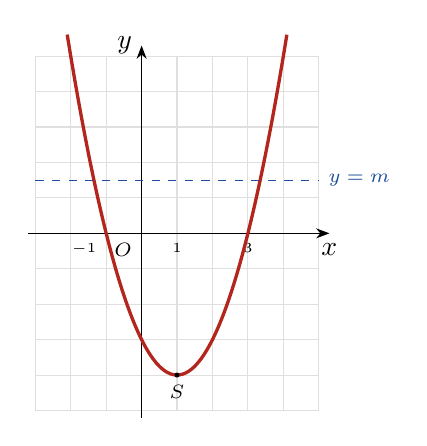
\begin{tikzpicture}[scale=0.45]
 \Grid{-3}{5}{-5}{5}
 \foreach \t in {1,3} \node[below,font=\tiny] at (\t,0){$\t$};
 \node[below left,font=\tiny] at (-1,0){$-1$};
 \draw[cThm,very thick,smooth,samples=60,domain=-2.1:4.1] plot (\x,{\x*\x-2*\x-3});
 \draw[cDef,dashed] (-3,1.5)--(5,1.5) node[right,font=\scriptsize]{$y=m$};
 \fill (1,-4) circle (2pt) node[below,font=\scriptsize]{$S$};
\end{tikzpicture}
\end{LTR}
\end{minipage}
\begin{enumerate}\setcounter{enumi}{3}
\item القيمة الحدية الصغرى لـ $f$ هي $-4$ (رأس القطع $S(1;-4)$):
\begin{itemize}
\item إذا كان $m<-4$: لا توجد حلول.
\item إذا كان $m=-4$: حل وحيد $x=1$.
\item إذا كان $m>-4$: حلان متمايزان.
\end{itemize}
\item $D_k=\{x:\ f(x)\ge0\}=\boxed{]-\infty;-1]\,\cup\,[3;+\infty[}$.\\
$k=\sqrt{\ }\circ f$ والدالة الجذر متزايدة تماماً، إذن لـ $k$ نفس اتجاه تغير $f$:
$k$ متناقصة تماماً على $]-\infty;-1]$ ومتزايدة تماماً على $[3;+\infty[$.
\end{enumerate}
\end{hal}

\begin{tamrin}{شامل (2)}
$f$ الدالة المعرفة على $\R-\{1\}$ بـ: $f(x)=\dfrac{2x+1}{x-1}$.
\begin{enumerate}
\item بيّن أنه من أجل كل $x\ne1$: \ $f(x)=2+\dfrac{3}{x-1}$.
\item استنتج اتجاه تغير $f$ على كل من المجالين $]-\infty;1[$ و $]1;+\infty[$.
\item بيّن أن النقطة $\Omega(1;2)$ مركز تناظر لـ $(C_f)$.
\item حل في $\R-\{1\}$ المعادلة $f(x)=x$ ، وفسّر النتيجة بيانياً.
\end{enumerate}
\end{tamrin}
\begin{hal}
\begin{enumerate}
\item $2+\dfrac{3}{x-1}=\dfrac{2(x-1)+3}{x-1}=\dfrac{2x+1}{x-1}=f(x)$.
\item $x\mapsto\dfrac{1}{x-1}$ متناقصة تماماً على كل من المجالين (مركب $x-1$ المتزايدة و $\dfrac1x$ المتناقصة) ،
والضرب في $3>0$ وإضافة $2$ لا يغيران الاتجاه: $f$ \textbf{متناقصة تماماً} على $]-\infty;1[$ وعلى $]1;+\infty[$.
\item $f(1+x)+f(1-x)=2+\dfrac3x+2-\dfrac3x=4=2\times2$ ، إذن $\Omega(1;2)$ مركز تناظر لـ $(C_f)$.
\item $\dfrac{2x+1}{x-1}=x\iff2x+1=x^2-x\iff x^2-3x-1=0$ ؛ \ $\Delta=13$:
\[x_1=\frac{3-\sqrt{13}}{2}\approx-0{,}30\qquad;\qquad x_2=\frac{3+\sqrt{13}}{2}\approx3{,}30\]
وكلاهما يختلف عن $1$. بيانياً: $(C_f)$ يقطع المستقيم $y=x$ في نقطتين فاصلتاهما $x_1$ و $x_2$.
\end{enumerate}
\end{hal}

\vfill
\begin{center}
{\color{cSec}\large\bfseries بالتوفيق والنجاح}
\end{center}
\end{document}
